
\subsection{MNIST dataset}

We tested RSOM on the standard MNIST dataset \citep{Lecun:1998} that contains $60,000$ training images and $10,000$ testing images. The dimension of each image is 28$\times$28 pixels and they are encoded using grayscale levels as the result of the normalization of the original black and white NIST database. The standard performance on most algorithms on the MNIST dataset is below 1\% error rate (with or without preprocessing) while for the regular SOM it is around 90\% recognition rate depending on the initial size, learning rate, and neighborhood function. Our goal here is not to find the best set of hyper-parameters but rather to explore if SOM and RSOM are comparable for a given set of hyper-parameters. Consequently, we considered a size of 32$\times$32 neurons and used the entire training set (60,000 examples) for learning and we measured performance on the entire testing set. We did not use any preprocessing stage on the image and we fed directly each image of the training set with the associated label to the model. Labels (from 0 to 9) have been transformed to a binary vector of size 10 using one-hot encoding (e.g. label 3 has been transformed to 0000001000). These binary labels can then be learned using the same procedure as for the actual sample. To decode the label associated to a code word, we simply consider the argmax of these binary vectors. Figure \ref{fig:MNIST:results} shows the final self-organisation of the RSOM where the class for each cell has been colorized using random colors. We can observe a number of large clusters of cells representing the same class (0, 1, 2, 3, 6) while the other classes (4,5,7,8,9) are split in two or three clusters. Interestingly enough, the codewords at the borders between two clusters are very similar. In term of recognition, this specific RSOM has an error rate just below 10\% ($0.903,\, \pm 0.296$) which is quite equivalent to the regular SOM error rate ($0.906,\, \pm 0.292$). The perfomances of the RSOM and SOM are actually not significantly different, suggesting that the regular grid hypothesis can be weaken.

In a similar way we measured the similarity of the neural spaces generated by both the regular SOM and the RSOM using the persistent diagram and barcodes. The only significant difference from previous analysis was the projection of the input and neural spaces to a lower-dimension space via UMAP \citep{Mcinnes:2018}. Projections of high-dimensional spaces to lower-dimension ones have been used before in the analysis of latent spaces of autoencoders \citep{Detorakis:2019}. Here, we use the UMAP since it's an efficient and robust method for applying a dimensionality reduction on input and neural spaces. More precisely, we project the MNIST digits as well as the code words (dimension $784$) to a space of dimension $7$. Once we get the projections, we proceed to the topological analysis using the persistent diagram and barcodes as we already have described in previous paragraphs.
Figure~\ref{fig:MNIST:analysis} shows the results regarding the persistent barcodes and diagrams. 
The persistent barcodes in figures~\ref{fig:MNIST:analysis}A, B, and C indicate that RSOM captures more 
persistent features (panel C, orange and green lines reflect the $H1$- and $H2$-homological features, respectively)
than the regular SOM (panel B). The persistence diagrams of input, SOM and RSOM are shown in 
figures~\ref{fig:MNIST:analysis} D, E, and F, respectively. 
These figures indicate that the RSOM has more persistent features (orange and green dots away from the diagonal
line) than the regular SOM, consistently with the two previous experiments ($2$D uniform distribution with holes
and $3$D uniform distribution). The Bottleneck distance between the persistence diagrams of input space and 
those of SOM and RSOM for the $H0$ are SOM: $1.0$ and RSOM: $1.12$, for $H1$ SOM: $0.19$ and RSOM: $0.22$, and
finally for the $H2$ are SOM: $0.05$ and RSOM:$0.05$. Again we observe that the regular SOM has a persistent 
diagram that is closer to the one of the input space than that of RSOM, however the RSOM seems to approache 
slightly better the input space topology since it has more pairs (birth, death) away from the diagonal (black
line) in figures~\ref{fig:MNIST:analysis}D, E, and F. Moreover, the persistent barcode of RSOM (figure~\ref{fig:MNIST:analysis}C indicates that has more persistent features for the radius $\alpha$
between $0$ and $1.512$ than the regular SOM.

\begin{figure}
  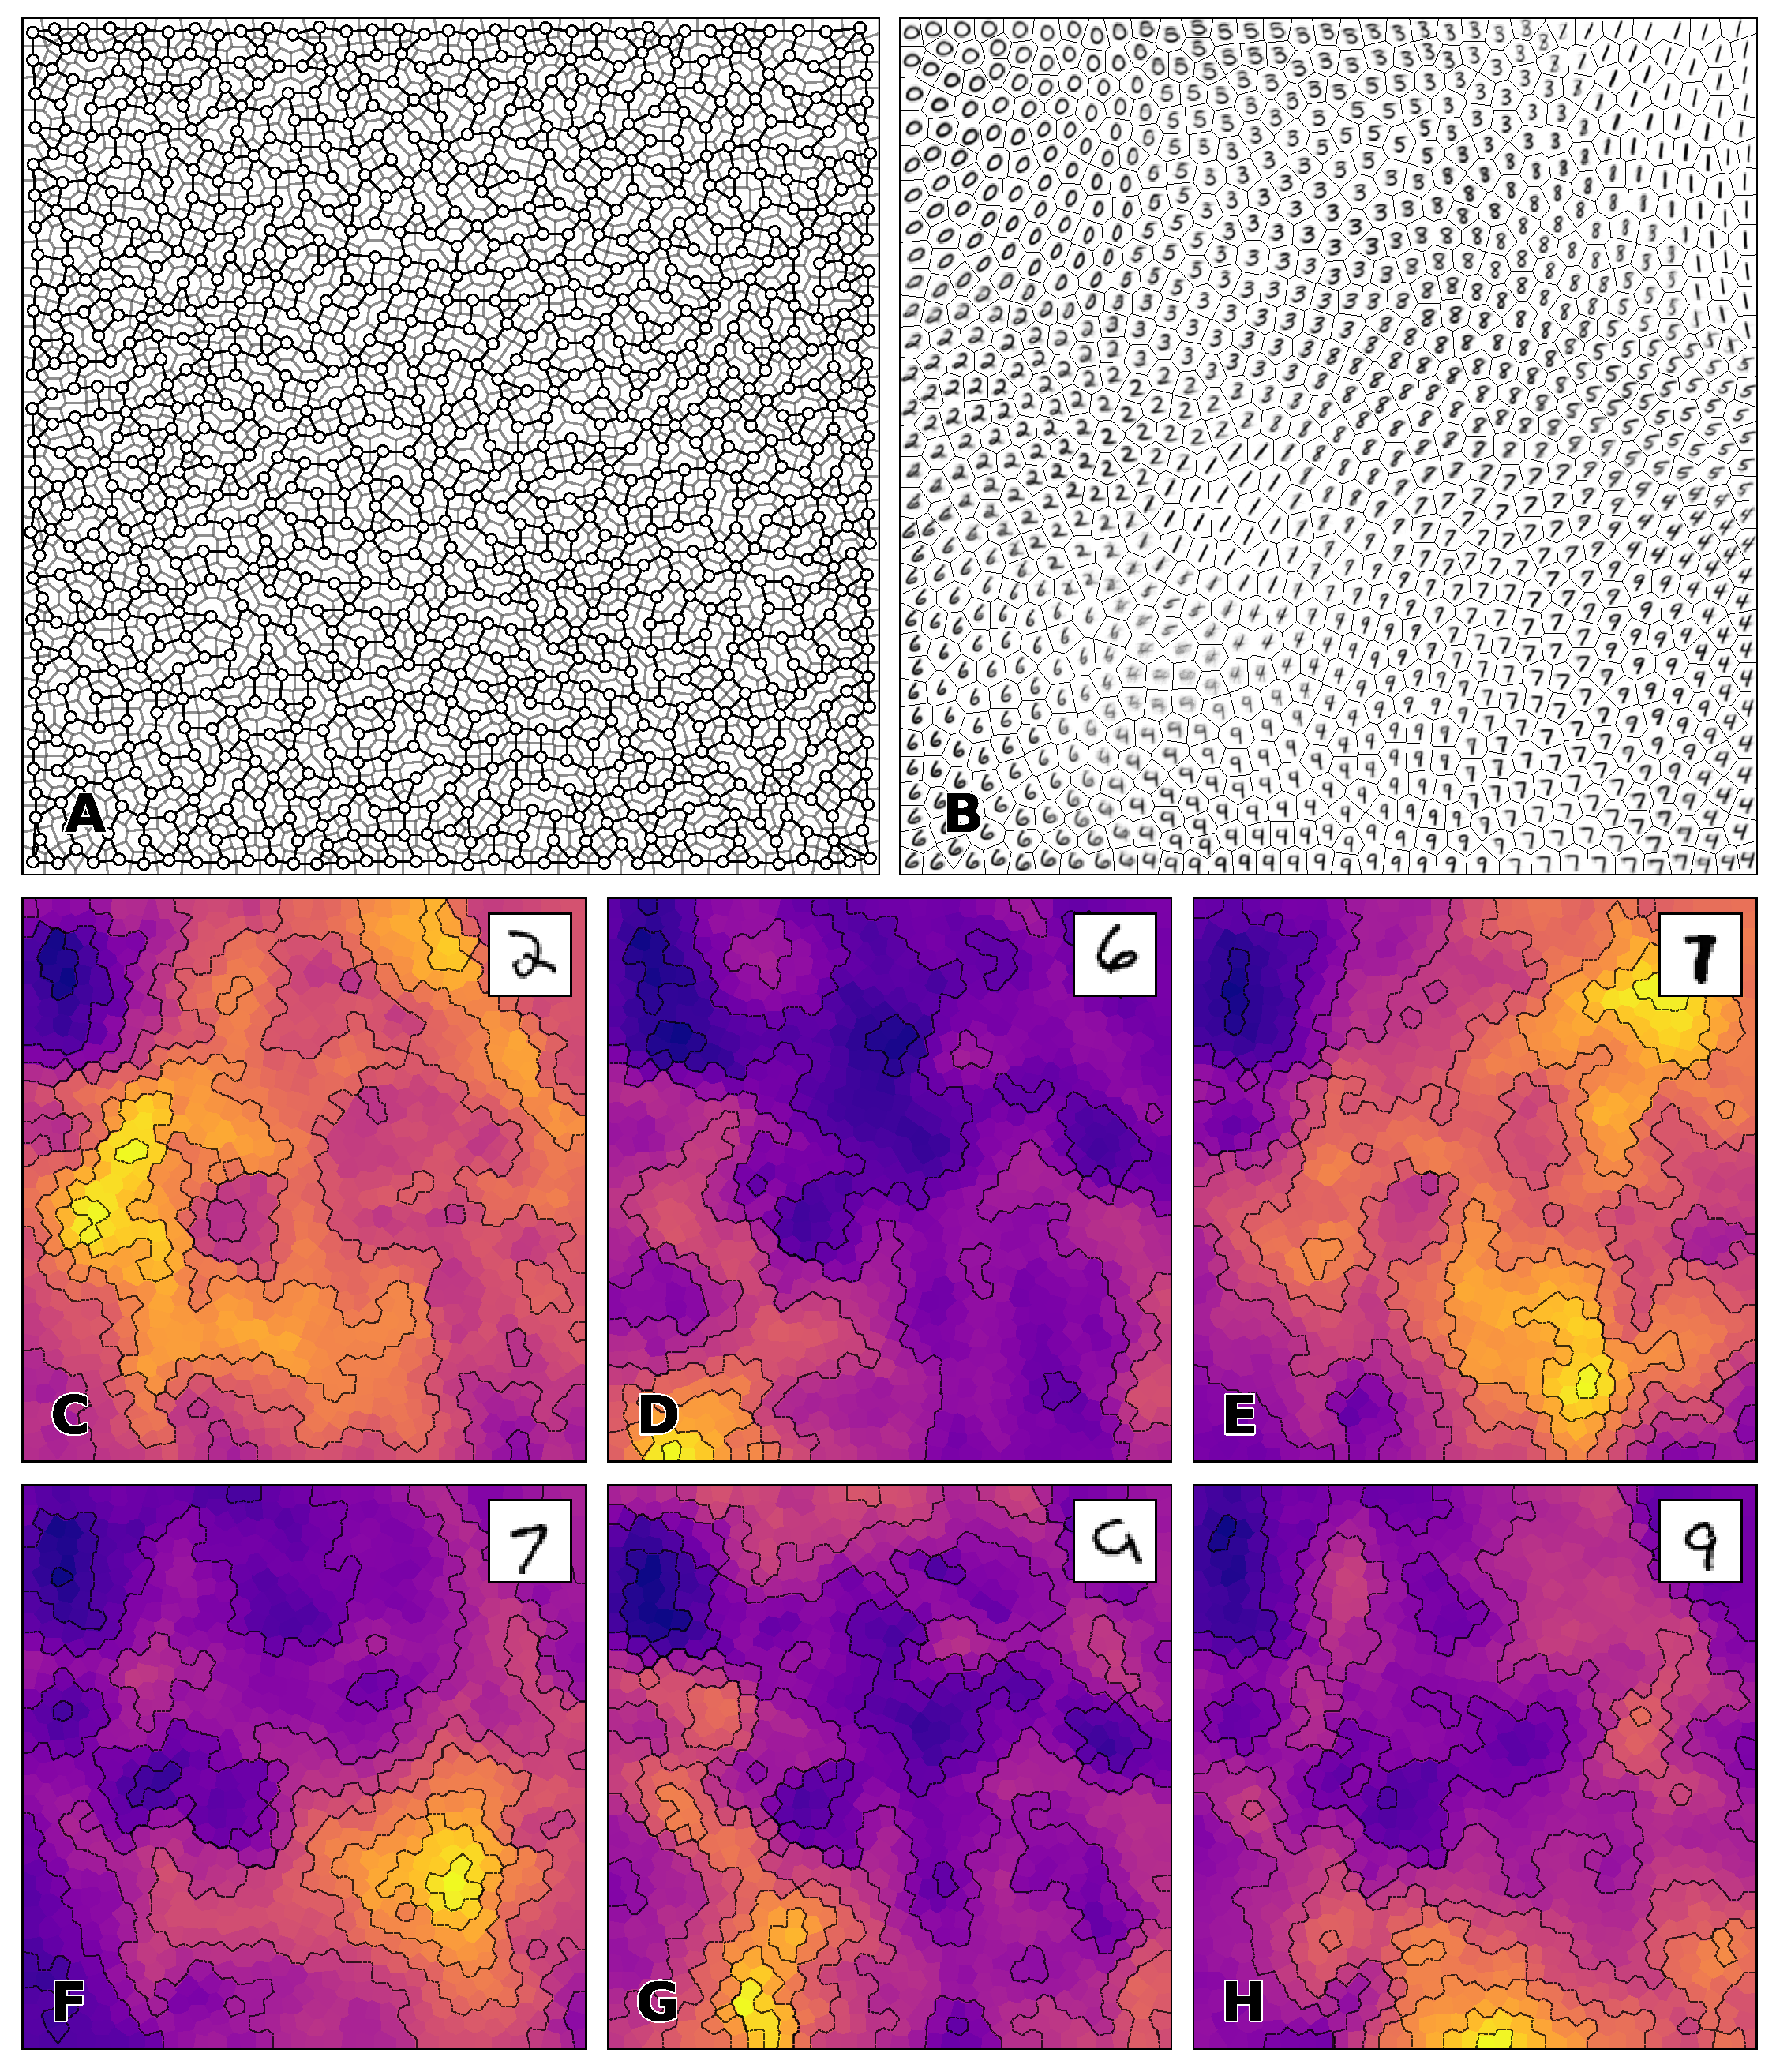
\includegraphics[width=\columnwidth]{experiment-MNIST.pdf}
  \vspace{2mm}
  \centering
  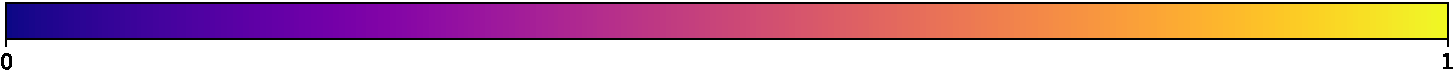
\includegraphics[width=.975\columnwidth]{figures/colormap.pdf}
  %
  \caption{%
  %
  {\bfseries \sffamily MNIST dataset (results)}
  %
  Randomized SOM made of $1024$ neurons with a $3$-nearest neighbors induced topology. Model has been trained for $25,000$ epochs on the MNIST dataset. \textbf{A} Map topology in neural space. \textbf{B} Map topology in data space. \textbf{C to H} Normalized distance map for six samples. Normalization has been performed for each sample in order to enhance contrast but this prevents comparison between maps.
  %
  }
  \label{fig:MNIST:results}
\end{figure}


\begin{figure}
  \centering
  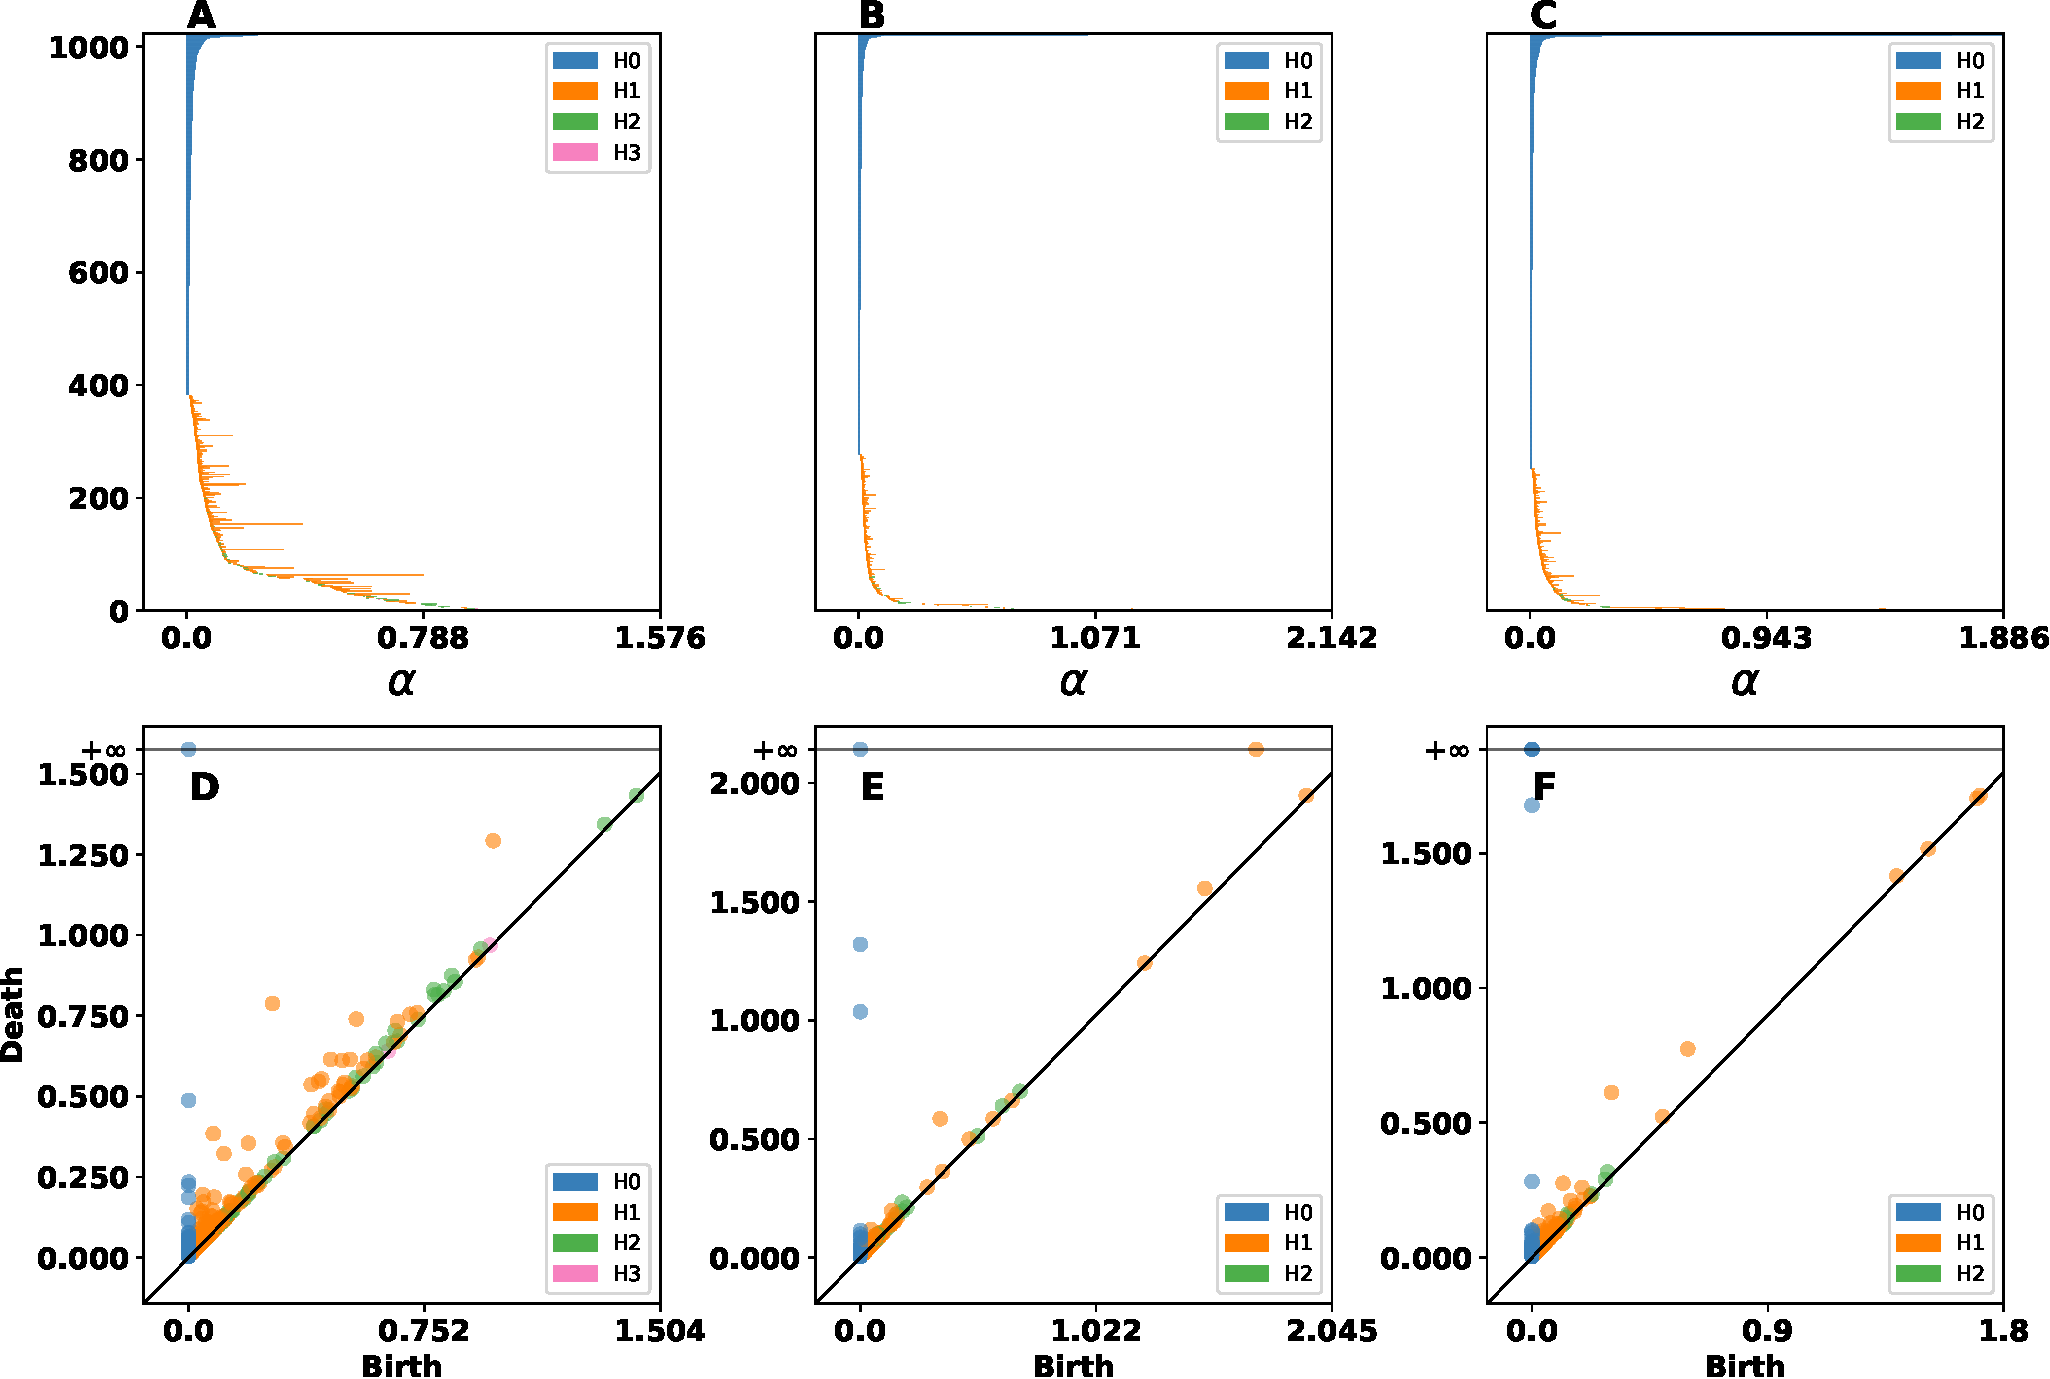
\includegraphics[width=\textwidth]{experiment-MNIST-analysis.pdf}
  \caption{{\bfseries \sffamily MNIST dataset (analysis)}
  Persistent Barcodes of \textbf{A} input space, \textbf{B} SOM, and \textbf{RSOM}.
  The blue, orange, and green line segments represent the $H0$-, $H1$-, and $H2$-homology,
  respectively. This means
  that blue color represents connected segments within the space, orange color reflects the holes
  within the space and green the voids. The longer the line segment the more important the 
  corresponding topological feature. \textbf{D} illustrates the persistent diagram for the input space.
  \textbf{E} and \textbf{F} depict the persistent diagrams for SOM and RSOM, respectively. Again blue dots
  indicate $H0$-homology features, orange dots represent $H1$-homolocical features, and green the 
  $H2$-homological features.}
  \label{fig:MNIST:analysis}
\end{figure}